\chapter{LND instrument}
\label{chp:LNDinstrument}

\section{LND simulation}
\label{chp:LNDsimulation}
The screen shot of the LND structure and 

\section{temperature variation of the LND instrument from 2019 to 2023}

Inside of the sensor head, LND has several temperature measusment sensor, monitoring the temperature variation of the chips and the surrounding temperature, as shown in Fig.\ref{}. The temperature sensor only operates together with LND on the day time. 
The temperature variation on the lunar surface

\begin{figure}
    \centering
    \subfloat[]{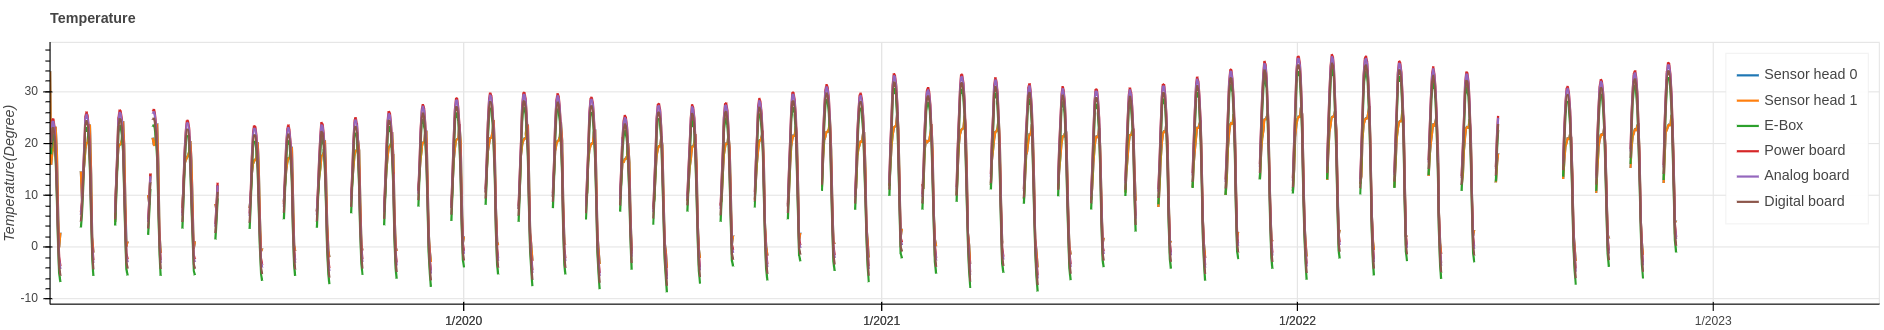
\includegraphics[angle = 90, width = 0.30\textwidth, height = \textheight]{images/lnd_temperature.png}}
    \subfloat[]{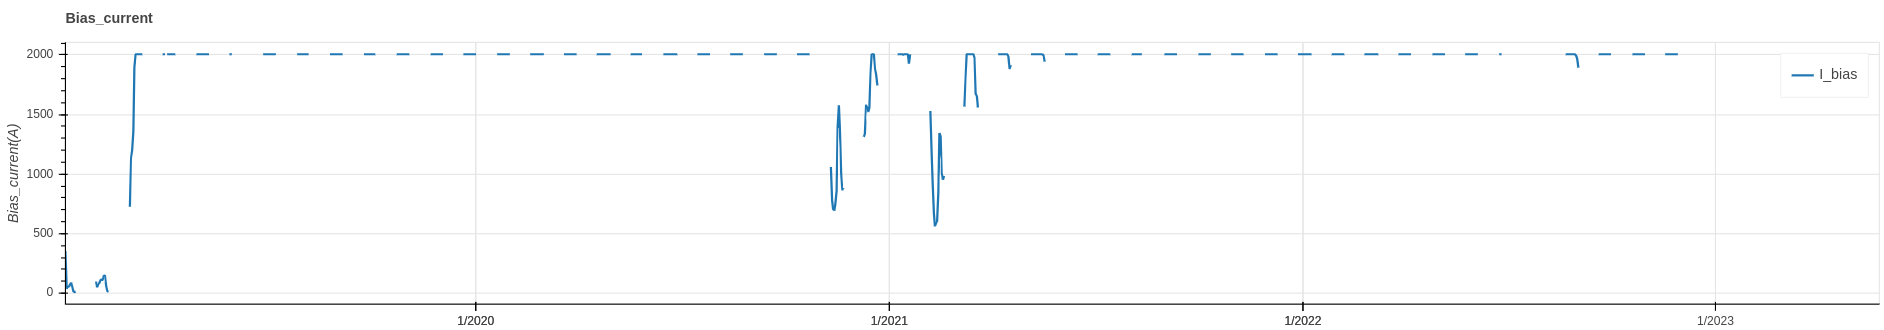
\includegraphics[angle = 90, width = 0.25\textwidth, height = \textheight]{images/lnd_bias_current.png}}
    \subfloat[]{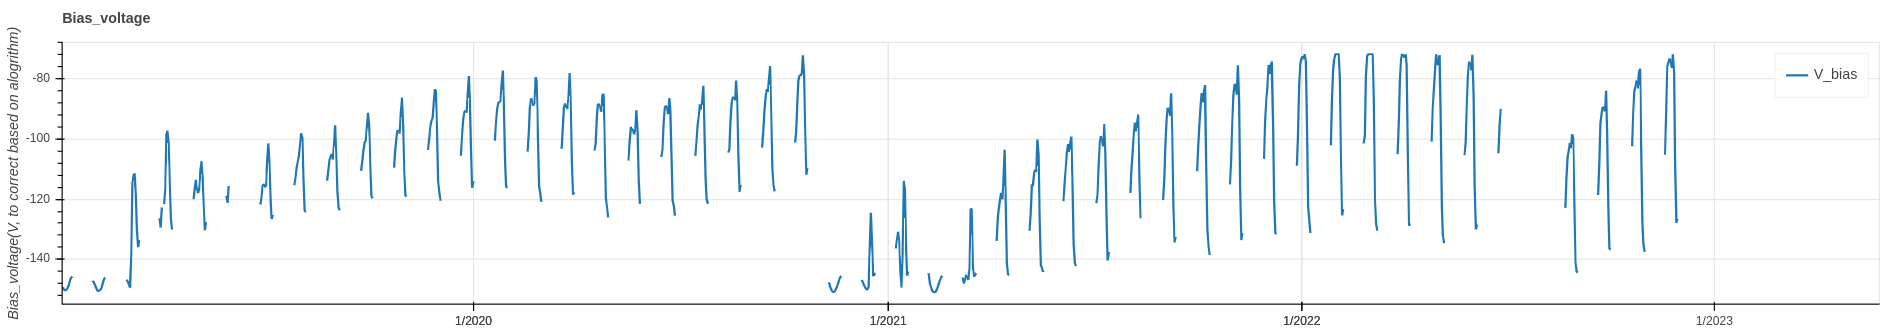
\includegraphics[angle = 90, width = 0.25\textwidth, height = \textheight]{images/lnd_bias_voltage.png}}
    \caption[LND temperature, bias current, and bias voltage variations]{The variation of housekeeping data including (a) temperature, (b) bias current, and (c) bias voltage. The temperatures are measured by the sensors assembled inside of LND sensor head and electronic box. The overview plot  2019 to Nov 29, 2022. }
    \label{Fig:appendix_LND_Housekeeping}
\end{figure}

\section{The overall proton, helium and TID variation and the most updated SEP list}

\begin{figure}
    \centering
    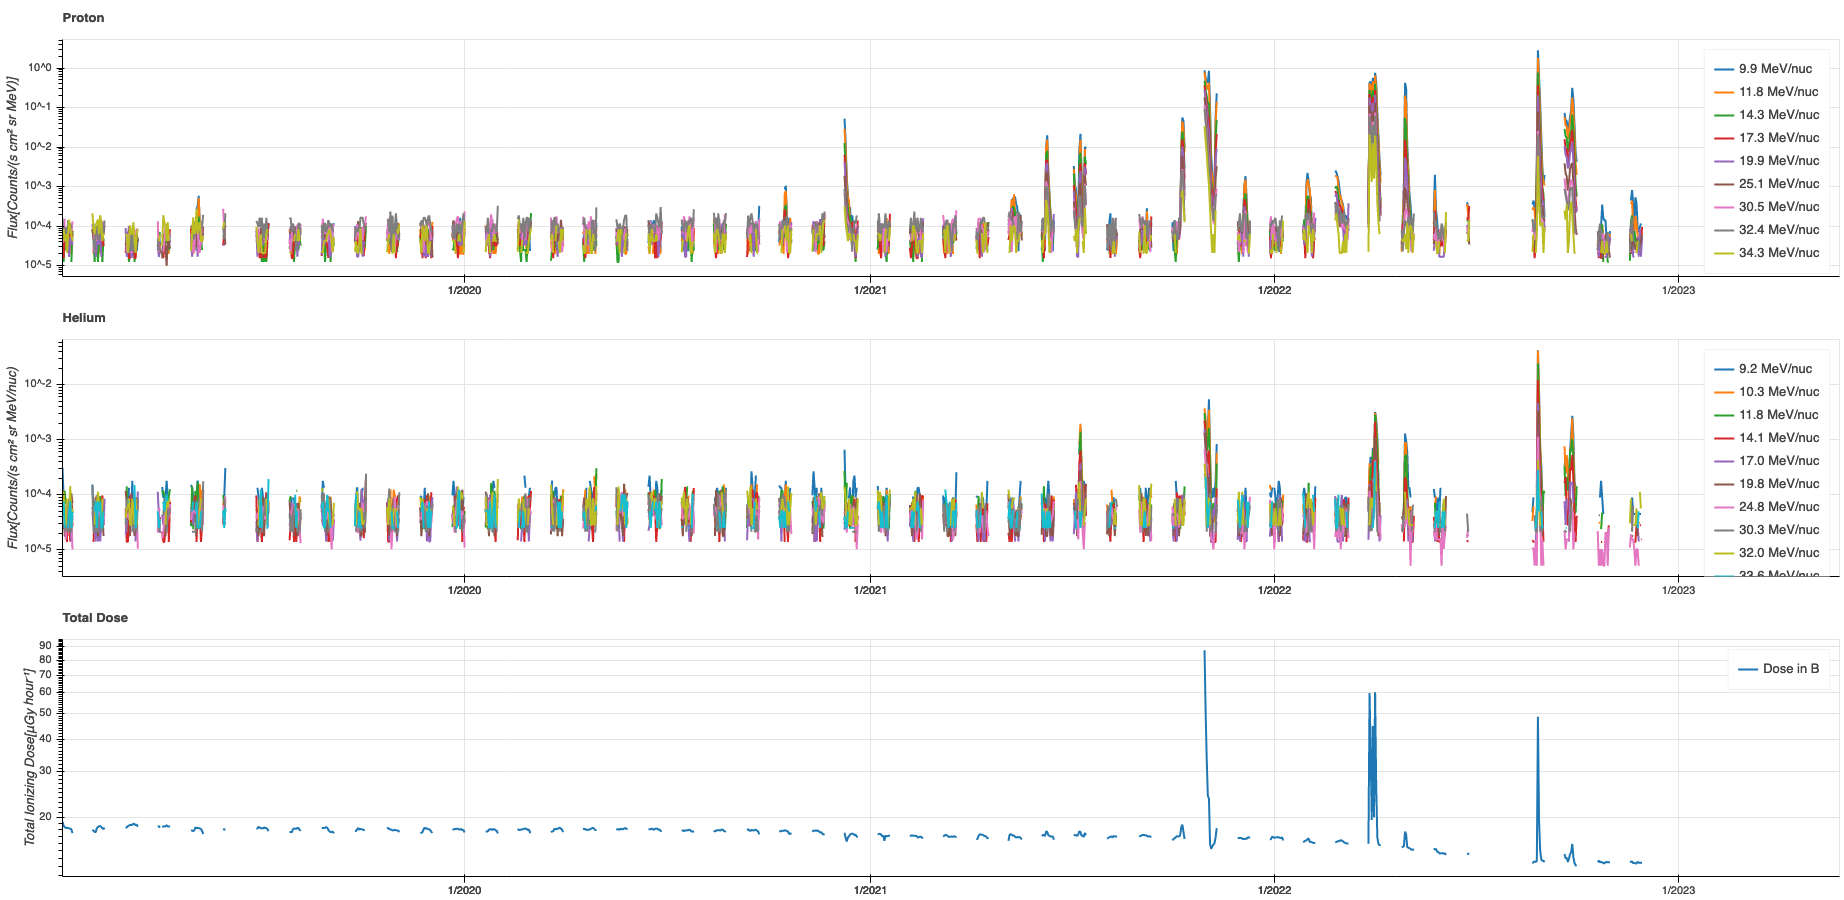
\includegraphics[angle = 90, width =0.8\textwidth, height = \textheight]{images/LND-proton-helium-TID.png}
    \caption[The overview of proton, helium flux and \ac{TID} measured by \ac{LND}]{The proton, helium flux and \ac{TID} temporal variation from 2019 to Nov 29, 2022, measured by \ac{LND} on the lunar far-side surface}
    \label{Fig:appendix_LND_proton_helium_TID}
\end{figure}
\clearpage
The above figures are generated by the LND webplotter which is a web application that is used to visualize the LND measurement in a quick and fast way. 
Currently, the webplotter is running in a server named etsasa located in the IEAP.
The webplotter is written in Python and the source code is available in the github repository \url{https://gitlab.physik.uni-kiel.de/LND/lnd_webplotter}. 
Inner used webplotter 
Created by Zigong Xu. following the tempelate of SOLO loader

2021 August, Lid problem. Beside, malfunction of the LND lid.

% create a table of SEP list that LND measured
\begin{table}[!h]
    \centering
    \caption[The SEP event list observed on LND]{The SEP event list observed on LND between 2019 and 2022}
\begin{tabular}{cccccc}
    \hline
    No.     & Lunar day & Start time    & End time      & Radiation hazard  & Peak energy (proton)\\
    \hline
    1       & 5         &  2019-05-04 12:00 & 05-06 00:00               & N  & $\sim$ 10 MeV\\
    2       & 5         &  2019-05-06 06:00 & 05-06 18:00              & N  & $\sim$ 20 Mev \\
    3       & 1         &  2019-10-16 18:00 & 10-19 00:00             & N  & $\sim$ 20 MeV\\
    4       & 1         &  2019-12-09 06:00 & 12-12 00:00             & N  & $>$ 35 MeV\\    
    5       &           &  2021-06-09 06:00 & 06-12 00:00             & Y  & $>$ 35 MeV\\
    6       &           &  2021-07-04 06:00 & 07-07 00:00             & N  & $>$ 35 MeV\\
    7       &           &  2021-07-09 10:00 & 07-12 06:00             & Y  & $>$ 35 MeV\\
    8       &           &  2021-07-13 12:00 & 07-15 06:00             & Y  & $>$ 35 MeV\\
    9       &           &  2021-10-09 06:00 & 10-12 00:00             & Y  & $>$ 35 MeV\\
    10      &           &  2021-10-30 08:00 & 11-06 05:00             & Y(intensive)  & $>$ 35 MeV\\
    11      &           &  2021-11-09 10:00 & 11-10 08:00             & Y  & $\sim$ 30 MeV\\
    12      &           &  2021-12-05 05:00 & 12-07 09:00             & N  & $\sim$ 30 MeV\\
    13      &           &  2022-01-29 22:00 & 02-03 11:00             & N  & $\sim$ 30 MeV\\
    14      &           &  2022-02-25 06:00 & 03-01 19:00             & N  & $\sim$ 30 MeV\\
    15(a,b,c)      &           &  2022-03-28 06:00 & 04-07 01:00             & Y(intensive)  & $>$ 35 MeV\\
    16     &           &  2022-04-28 00:00 & 05-04 06:00             & Y  & $\sim$ 30 MeV\\
    17      &           &  2022-05-25 16:00 & 05-26 23:00             & N  & $\sim$ 20 MeV\\
    18      &           &  2022-08-26 08:00 & 09-01 11:00             & Y(intensive)  & $>$ 35 MeV\\
    19      &           &  2022-09-19 23:00 & 09-39 00:00             & Y  & $\sim$ 30 MeV\\
    20      &           &  2022-11-19 10:00 & 11-20 10:00             & N  & $\sim$ 15 MeV\\
    \hline
\end{tabular}
\label{Tab:appendix_LND_SEP_list}
\end{table}

The start time and end time are determined by the eye and have larger uncertainty. 

\section{Correction of the LND bias current and voltage}

Due to the noise of the detectors, the bias current reach the limit of the meaurements at 2$\mu$A. 

Below are the scripts used to calculate the correct bias voltage and current that measured on the LND instrument from Stephan B¨ottcher (private communication), who is the desinger of the LND instruement hardware and software in the IEAP.
\begin{lstlisting}[language=Python]
function Ibias() {
    a = $(HK_Ibias+3)
    if (a>4000) a = (147.3 + degC($(HK_T_LVPS+3))*0.164 - $(HK_Vbias+3)*0.05488) / 0.01810
    return a*0.4928
}

function Vbias() {
    return $(HK_Vbias+3)*0.05488 + $(HK_Ibias+3)*0.01810
}

\end{lstlisting}

\section{The change of \ac{LND} data process pipeline}
\label{chp:appendix_LND_data_process_pipeline}

\section{Discrepanchy between LND and CREME}

\section{Heavy ion spectra}

\section{He3 spectra}
\label{chp:appendix_LND_He3_spectra}
Mostly the instrument effect, the He3 spectra is not reliable.

\section{L1 responce simulation}

